\section{Sensor data naar pH omzetten}

\subsection*{Uitlezen ISFET}

    \begin{frame}
        \frametitle{Principe schakeling}
    
        \begin{figure}
            \centering
            \def\svgwidth{0.6\textwidth}
            \input{ISFETCircuitBest.pdf_tex}
        \end{figure}
    
    \end{frame}
    \begin{frame}
        \frametitle{Ruis analyse}
    
        \begin{figure}
            \centering
            \def\svgwidth{0.6\textwidth}
            \input{ISFETCircuitBestNoise.pdf_tex}
        \end{figure}
        \begin{equation}\label{eq:measureNoiseOut}
            S_{u_{{n,out}}} = \left(S_{u_{{n,ref}}} + S_{u_{{n,n}}} + S_{i_{{n,in}}}\left(Z_{fet} // R\right)^2\right) \cdot H^2(\ph)
        \end{equation}
    
    \end{frame}
    \begin{frame}
        \frametitle{Energie}

        $U_{dd}=3v3$

        \noindent
        $I_{ds}=50\mu$A
    
        \begin{equation}\label{eq:measurePower}
            P_{statisch} = P_{n,quiescent} + U_{dd}I_{ds}
        \end{equation}

        \pause

        \begin{equation}
            P_{statisch} = P_{n,quiescent} + 165\mu\mathrm{W}
        \end{equation}
    
    \end{frame}

    \subsection*{ADC}
    \begin{frame}
        \frametitle{Eisen}
    
        \begin{table}[ht]
    \centering
    \begin{tabular}{l|c|l}
        Symbol      & Waarde & Eenheid\\\hline
        $SNR_{in}$  & 37        & dB\\
        NF          & 3         & dB\\
        $u_{in}$    & 2.5       & mV\\
    \end{tabular}
    \caption{De eisen voor het omzetten van het analoge signaal naar een digitaal signaal.}
    \label{tab:systemSpecADC}
\end{table}
    
    \end{frame}
    \begin{frame}
        \frametitle{Minimum aantal bits}
        \centering

        De toelaatbare fout ten gevolge van de eindige resolutie van de ADC
        \begin{equation}\label{eq:calcSpecifiedRmsError}
            \overline{e_{eff}^2}=\left(10^{\frac{NF}{10}}-1\right)\left(\frac{S_{rms}}{10^{\left(SNR+NF\right)/20}}\right)^2
        \end{equation}
        \pause

        Berekenen minimum benodigde ADC resolutie
        \begin{equation}\label{eq:calcNeededQ}
            Q=\sqrt{12\cdot\overline{e_{eff}^2}}
        \end{equation}
        \pause

        Berekenen minimum aantal bits van de ADC op basis van de minimaal benodigde ADC resolutie 
        \begin{equation}\label{eq:calcMinNumberADCbits}
            n=\left\lceil\log_2\left(\frac{1}{Q}+1\right)\right\rceil=14
        \end{equation}
    
    \end{frame}

    \begin{frame}
        \frametitle{Sample frequentie}
        \centering
        
        Toelaatbare fout
        \begin{equation}\label{eq:ADCmaxSampleError}
            E=10^{\frac{-NF}{10}}
        \end{equation}
        \pause

        Minimale sample frequentie berekenen
        \begin{equation}\label{eq:ADCminFs}
            f_{s,min}=\frac{\pi f_h}{E}=45
        \end{equation}
    
    \end{frame}

    \subsection*{AA filter}
    \begin{frame}
        \frametitle{Eisen anti aliasing filter}
        
        \centering

        Dempen 22.5Hz


        $P_{max}=200\mu$W


        $NF=3\si{\decibel}$
        \vspace{2cm}


        \pause

        \begin{figure}
            \centering
            \def\svgwidth{0.4\textwidth}
            \subsection{Filter}
Tussen de ADC en de uitleesschakeling van de sensor zit een filter. Dit filter zorgt ervoor dat alle frequenties buiten de bandbreedte weggefilterd worden. Er is gekozen om hiervoor een eerste orde filter te gebruiken.
De schakeling van dit filter is te zien in \autoref{fig:filterCircuit}. De kantelfrequentie het filter ligt aan de waardes van $C$ en $R$, volgens \autoref{eq:cutoffFreq}.

\subsubsection{Ruis}
De spectrale ruisdichtheid aan de ingang van het filter is te berekenen met \autoref{eq:filterNoiseDensity}.
De spectrale ruisdichtheid aan de uitgang van het filter is hetzelfde als die van de spanningsdeler in \autoref{sec:referenceVoltage}. Deze is te berekenen met \autoref{eq:dividerNoise}.

\begin{figure}[ht]
    \centering
    \def\svgwidth{0.3\textwidth}
    \subsection{Filter}
Tussen de ADC en de uitleesschakeling van de sensor zit een filter. Dit filter zorgt ervoor dat alle frequenties buiten de bandbreedte weggefilterd worden. Er is gekozen om hiervoor een eerste orde filter te gebruiken.
De schakeling van dit filter is te zien in \autoref{fig:filterCircuit}. De kantelfrequentie het filter ligt aan de waardes van $C$ en $R$, volgens \autoref{eq:cutoffFreq}.

\subsubsection{Ruis}
De spectrale ruisdichtheid aan de ingang van het filter is te berekenen met \autoref{eq:filterNoiseDensity}.
De spectrale ruisdichtheid aan de uitgang van het filter is hetzelfde als die van de spanningsdeler in \autoref{sec:referenceVoltage}. Deze is te berekenen met \autoref{eq:dividerNoise}.

\begin{figure}[ht]
    \centering
    \def\svgwidth{0.3\textwidth}
    \subsection{Filter}
Tussen de ADC en de uitleesschakeling van de sensor zit een filter. Dit filter zorgt ervoor dat alle frequenties buiten de bandbreedte weggefilterd worden. Er is gekozen om hiervoor een eerste orde filter te gebruiken.
De schakeling van dit filter is te zien in \autoref{fig:filterCircuit}. De kantelfrequentie het filter ligt aan de waardes van $C$ en $R$, volgens \autoref{eq:cutoffFreq}.

\subsubsection{Ruis}
De spectrale ruisdichtheid aan de ingang van het filter is te berekenen met \autoref{eq:filterNoiseDensity}.
De spectrale ruisdichtheid aan de uitgang van het filter is hetzelfde als die van de spanningsdeler in \autoref{sec:referenceVoltage}. Deze is te berekenen met \autoref{eq:dividerNoise}.

\begin{figure}[ht]
    \centering
    \def\svgwidth{0.3\textwidth}
    \input{img/filter.pdf_tex}
    \caption{Het eerste-orde filter.}
    \label{fig:filterCircuit}
\end{figure}

% TODO: BEPAAL OVERDRACHT

\begin{equation} \label{eq:cutoffFreq}
    2\pi f_c = \omega_c = \frac{1}{RC}
    \tagaddtext{[\si{\radian\per\second}]}
\end{equation}

% \begin{equation} \label{eq:filterTransfer}
%     H(s) = \frac{1}{1+sRC}
% \end{equation}

\begin{equation} \label{eq:filterNoiseDensity}
    S_{u_{in}} = 4kTR
    \tagaddtext{[\si{\volt\squared\per\hertz}]}
\end{equation}

% De signaal-ruis verhouding aan de uitgang van dit filter is te berekenen met \autoref{eq:filterSNR}
% \begin{equation}\label{eq:filterSNR}
%     \mathrm{SNR} = 20\log\left(U_{out,min}\sqrt{\frac{C}{kT}}\right)
%     \tagaddtext{[\si{\decibel}]}
% \end{equation}

\subsubsection{Vermogen}
Het vermogensverbruik van het filter is te berekenen met \autoref{eq:filterPowerLaplace}.
\begin{equation} \label{eq:filterPowerLaplace}
    P = \frac{U_{in,max}^2}{\left|R + \frac{1}{sC}\right|}
    \tagaddtext{[\si{\watt}]}
\end{equation}
Omdat volgens \autoref{eq:cutoffFreq} $R$ te definiëren is in $\omega_c$ en $C$, volgt hieruit \autoref{eq:filterPower}.
\begin{equation} \label{eq:filterPower}
    P = \frac{1}{\sqrt{2}}\omega_cCU_{in,max}^2
    \tagaddtext{[\si{\watt}]}
\end{equation}
Uit deze formule is te zien dat het vermogensverbruik lineair evenredig is met de condensatorwaarde. Om het vermogensverbruik te minimaliseren moet dus een zo klein mogelijk condensatorwaarde gekozen worden. Aangezien de noise-figure van dit filter maximaal 3dB mag zijn, mag dit filter maximaal evenveel spanningsruis genereren als het systeem ervoor. Hieruit volgt \autoref{eq:dividerNoise}, waarmee de minimale condensatorwaarde te berekenen is. Hierbij is $u_{n,in}$ de ruisspanning aan de ingang van het filter.
\begin{equation} \label{eq:filterCapMin}
    C_{min} = \frac{kT}{u_{n,in}^2}
    \tagaddtext{[\si{\farad}]}
\end{equation}
    \caption{Het eerste-orde filter.}
    \label{fig:filterCircuit}
\end{figure}

% TODO: BEPAAL OVERDRACHT

\begin{equation} \label{eq:cutoffFreq}
    2\pi f_c = \omega_c = \frac{1}{RC}
    \tagaddtext{[\si{\radian\per\second}]}
\end{equation}

% \begin{equation} \label{eq:filterTransfer}
%     H(s) = \frac{1}{1+sRC}
% \end{equation}

\begin{equation} \label{eq:filterNoiseDensity}
    S_{u_{in}} = 4kTR
    \tagaddtext{[\si{\volt\squared\per\hertz}]}
\end{equation}

% De signaal-ruis verhouding aan de uitgang van dit filter is te berekenen met \autoref{eq:filterSNR}
% \begin{equation}\label{eq:filterSNR}
%     \mathrm{SNR} = 20\log\left(U_{out,min}\sqrt{\frac{C}{kT}}\right)
%     \tagaddtext{[\si{\decibel}]}
% \end{equation}

\subsubsection{Vermogen}
Het vermogensverbruik van het filter is te berekenen met \autoref{eq:filterPowerLaplace}.
\begin{equation} \label{eq:filterPowerLaplace}
    P = \frac{U_{in,max}^2}{\left|R + \frac{1}{sC}\right|}
    \tagaddtext{[\si{\watt}]}
\end{equation}
Omdat volgens \autoref{eq:cutoffFreq} $R$ te definiëren is in $\omega_c$ en $C$, volgt hieruit \autoref{eq:filterPower}.
\begin{equation} \label{eq:filterPower}
    P = \frac{1}{\sqrt{2}}\omega_cCU_{in,max}^2
    \tagaddtext{[\si{\watt}]}
\end{equation}
Uit deze formule is te zien dat het vermogensverbruik lineair evenredig is met de condensatorwaarde. Om het vermogensverbruik te minimaliseren moet dus een zo klein mogelijk condensatorwaarde gekozen worden. Aangezien de noise-figure van dit filter maximaal 3dB mag zijn, mag dit filter maximaal evenveel spanningsruis genereren als het systeem ervoor. Hieruit volgt \autoref{eq:dividerNoise}, waarmee de minimale condensatorwaarde te berekenen is. Hierbij is $u_{n,in}$ de ruisspanning aan de ingang van het filter.
\begin{equation} \label{eq:filterCapMin}
    C_{min} = \frac{kT}{u_{n,in}^2}
    \tagaddtext{[\si{\farad}]}
\end{equation}
    \caption{Het eerste-orde filter.}
    \label{fig:filterCircuit}
\end{figure}

% TODO: BEPAAL OVERDRACHT

\begin{equation} \label{eq:cutoffFreq}
    2\pi f_c = \omega_c = \frac{1}{RC}
    \tagaddtext{[\si{\radian\per\second}]}
\end{equation}

% \begin{equation} \label{eq:filterTransfer}
%     H(s) = \frac{1}{1+sRC}
% \end{equation}

\begin{equation} \label{eq:filterNoiseDensity}
    S_{u_{in}} = 4kTR
    \tagaddtext{[\si{\volt\squared\per\hertz}]}
\end{equation}

% De signaal-ruis verhouding aan de uitgang van dit filter is te berekenen met \autoref{eq:filterSNR}
% \begin{equation}\label{eq:filterSNR}
%     \mathrm{SNR} = 20\log\left(U_{out,min}\sqrt{\frac{C}{kT}}\right)
%     \tagaddtext{[\si{\decibel}]}
% \end{equation}

\subsubsection{Vermogen}
Het vermogensverbruik van het filter is te berekenen met \autoref{eq:filterPowerLaplace}.
\begin{equation} \label{eq:filterPowerLaplace}
    P = \frac{U_{in,max}^2}{\left|R + \frac{1}{sC}\right|}
    \tagaddtext{[\si{\watt}]}
\end{equation}
Omdat volgens \autoref{eq:cutoffFreq} $R$ te definiëren is in $\omega_c$ en $C$, volgt hieruit \autoref{eq:filterPower}.
\begin{equation} \label{eq:filterPower}
    P = \frac{1}{\sqrt{2}}\omega_cCU_{in,max}^2
    \tagaddtext{[\si{\watt}]}
\end{equation}
Uit deze formule is te zien dat het vermogensverbruik lineair evenredig is met de condensatorwaarde. Om het vermogensverbruik te minimaliseren moet dus een zo klein mogelijk condensatorwaarde gekozen worden. Aangezien de noise-figure van dit filter maximaal 3dB mag zijn, mag dit filter maximaal evenveel spanningsruis genereren als het systeem ervoor. Hieruit volgt \autoref{eq:dividerNoise}, waarmee de minimale condensatorwaarde te berekenen is. Hierbij is $u_{n,in}$ de ruisspanning aan de ingang van het filter.
\begin{equation} \label{eq:filterCapMin}
    C_{min} = \frac{kT}{u_{n,in}^2}
    \tagaddtext{[\si{\farad}]}
\end{equation}
        \end{figure}
    
    \end{frame}
    \begin{frame}
        \frametitle{Ruis \& vermogensanalyse RC filter}
    
        \begin{equation}\label{eq:dividerNoise}
            u_{n,out}^2 = \frac{kT}{C}
        \end{equation}

        \begin{equation} \label{eq:filterPower}
            P = \frac{1}{\sqrt{2}}\omega_cCU_{in,max}^2
        \end{equation}

        \pause

        \begin{equation} \label{eq:filterCapMin}
            C_{min} = \frac{kT}{u_{n,in}^2}
        \end{equation}

        \begin{equation}
            R = \frac{1}{2\pi fC}
        \end{equation}
    
    \end{frame}
    \begin{frame}
        \frametitle{AA filter}
    
        \begin{table}[ht]
            \centering
            \begin{tabular}{l|l|l}
                Symbool & Waarde & Eenheid \\
                \hline
                $C$         & 82    & $\si{\nano\farad}$\\
                $R$         & 180   & $\si{\kilo\ohm}$  \\
                $f_c$       & 10.8  & $\si{\hertz}$     \\
                $P$         & 408   & $\si{\nano\watt}$ \\
                $u_{n,out}$ & 225   & $\si{\nano\volt}$ \\
                NF          & 0.23  & $\si{\decibel}$   \\
            \end{tabular}
            \caption{De gekozen waardes van het filter, en de resulterende vermogens- en ruiseigenschappen.}
            \label{tab:filterValues}
        \end{table}
    
    \end{frame}
    \begin{frame}
        \frametitle{Effecten van de load}
    
        Spanningsdeler met de ADC, hierdoor wordt het ingangssignaal kleiner.
    
    \end{frame}

    \subsection*{Berekenen pH}
    \begin{frame}
        \frametitle{Gemeten waarde omrekenen naar pH}

        \begin{equation}\label{eq:digitaleBS}
            pH = C_{pH}(\
                \only<2>{\colorbox{yellow}{$U_{pH}$}}\only<1,3->{U_{pH}}\
            - U_{pH,kal}) + C_T(\
                \only<3>{\colorbox{yellow}{$U_T$}}\only<-2,4->{U_T}\
            - U_{T,kal}) + pH_{kal}\
        \end{equation}
        

        \pause[4]
        
        \begin{figure}
            \centering
            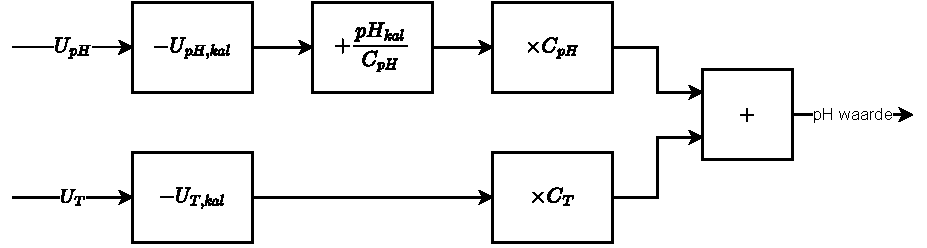
\includegraphics[width=\textwidth]{digitaleBewerkingsFunctie.pdf}
        \end{figure}
        % $\mathrm{CAL_{\mathrm{pH,H}}}=7$

        % $\mathrm{CAL_{\mathrm{pH,L}}}=4$

        % \begin{equation}
        %     \mathrm{pH}=\frac{\mathrm{S}-\mathrm{CAL_{\mathrm{ADC,L}}}}{\mathrm{CAL_{\mathrm{ADC,H}}}-\mathrm{CAL_{\mathrm{ADC,L}}}}\left(\mathrm{CAL_{\mathrm{pH,H}}}-\mathrm{CAL_{\mathrm{pH,L}}}\right)+\mathrm{CAL_{\mathrm{pH,L}}}
        % \end{equation}
    
    \end{frame}